\documentclass[oneside,10pt,a4paper]{report}
\usepackage[a4paper, left=3cm, right=3cm, top=3cm, bottom=3cm, headsep=10mm, footskip=12mm]{geometry}
\usepackage[T1]{fontenc}
\usepackage[ngerman, english]{babel}    % mehrsprachiger Textsatz
% babel: letzte Sprache in Optionen zeigt die Sprache des Dokumentes
% und kann durch den Befehl \selectlanguage{} geaendert werden
% Passen Sie die Optionen des babel-Paketes nach Bedarf an!
\usepackage{float}
\usepackage{graphicx}
\usepackage{url}
\usepackage{pdflscape}
\usepackage{mathtools}
\usepackage{amssymb, amsmath, amstext}
\usepackage{amsthm}
\usepackage{xcolor}
\usepackage{nameref}
\usepackage{siunitx}
\usepackage{makecell}
\usepackage{hyperref}
\usepackage{enumitem}
\usepackage[superscript,biblabel]{cite}
\usepackage{caption}
\usepackage{subcaption}
\usepackage{tabularx} 			% Tabellen erzeugen
\usepackage{multirow}			 % Zeilen in Tabellenbearbeitung
\usepackage{multicol} 			% Spalten in Tabellenbearbeitung 
\usepackage{lmodern}                        % Ersatz fuer Computer Modern-Schriften 
\usepackage{amsmath}                                           % zum besseren Aussehen am Bildschirm
\usepackage{booktabs} % für schönere Tabellen
\usepackage{sidecap}
\usepackage{rotating} % für die Landscape-Umgebung
\usepackage{afterpage}
\definecolor{Bluetitle}{HTML}{1F3864}
\definecolor{softbluetitle}{HTML}{274D7E}
\definecolor{Greyish}{HTML}{5A5A5A}
%\renewcommand{\refname}{Reference}
\usepackage{array,multirow}
\newcommand{\specialcell}[2][c]{%
	\begin{tabular}[#1]{@{}c@{}}#2\end{tabular}}
\usepackage{titlesec}

\titleformat{\chapter}[display]
{\normalfont\bfseries}{}{0pt}{\Huge}

\usepackage{lipsum} 


\begin{document}
	
	\begin{titlepage}
		
		
	
		
		\begin{center}
			\begin{figure}[h!tbp]
				
\includegraphics[width=\linewidth]{HUlogo.PNG}
			\end{figure}
		\end{center}
			
			
			\textcolor{Greyish}{\textbf{Lebenswissenschaftliche Fakultät}}\par
			\textcolor{Greyish}{Institut für Biologie}\par
			\textcolor{Greyish}{Institute for Theoretical Biology)}\par
			\vspace*{4 cm}
		\begin{center}
			
			\textcolor{softbluetitle}{\textbf{\Large Studienprojekt}}\par
			\vspace*{1 cm}
			\textcolor{Bluetitle}{\textbf{\Huge Implementing ODE Models for Biological Oscillators}}\par
			\vspace*{1 cm}
			\textcolor{softbluetitle}{\textbf{\Large Coupling Duffing and Van der Pol Oscillators}}\par
			
		\end{center}
			\vspace*{4cm}
		
			
			
			\vspace*{0.5cm}
			\textcolor{Greyish}{vorgelegt von}\par
			\vspace*{0.5cm}
			\textcolor{Greyish}{Huyen Anh Nguyen}\par
			\textcolor{Greyish}{Matrikelnummer 572309}\par
			\textcolor{Greyish}{huyen.anh.nguyen@student.hu-berlin.de}\par
			\textcolor{Greyish}{Geboren am 14.03.1996 in Strausberg}\par
			\vspace*{0.5cm}
			\textcolor{Greyish}{Erstprüfer:		Prof. Dr. Hanspeter Herzel}\par
			\textcolor{Greyish}{Zweitprüfer:		Dr. Mathias König}\par
			
			
			
	
	\end{titlepage}
	
	
	\tableofcontents
	\chapter{Motivation}
	
		Many people enjoy listening to music. And in the music scene, there are many genres from classical music to heavy metal music. Fascinating tones are produced daily, which we can perceive with our ears and process in our brains. The tones are transmitted as sound waves to our ears through air, water, or solids and are generated by various sound wave producers, such as the vocal folds.\\
		We can perceive and produce both linear and nonlinear phenomena. \\
		Especially the nonlinear phenomena are particularly interesting, not only how we can produced them, but also the mathematical background of it is interesting.\\
		 For example, the metal singer Daniel Priegnitz can produce linear oscillatory movement sounds with his vocal folds driven by subglottic pressure, but he can also produce nonlinear sounds using well-known metal vocal techniques like "growling" with his false vocal folds (also called ventricular folds) \cite{DanielPriegnitz}.
		 Driven by the skills of Daniel Priegnitz and the desire to understand nonlinear sound production, two oscillator models (the Duffing oscillator and the Van der Pol oscillator) are implemented into one oscillator model. Each oscillator contributes its own properties to this new system.\\
		 In this "Studienprojekt" I will explain the equations of the two chosen models (Duffing oscillator and Van der Pol oscillator) and try to understand how the period T, frequency f, and angular frequency $\omega$ will change for the new driven oscillator model. I will also analyze the amplitude response of the Duffing oscillator.\\
		 Although there are plenty of existing different models, the hope of this new model is to gain new insights into complex nonlinear sound production.\\
		
	\chapter{Duffing and Van der Pol Oscillator} \label{chapter: Duffing- and Van der Pol Oscillator}
	
		The Duffing and Van der Pol oscillators are both nonlinear oscillators, each with their own special properties. 
		The two oscillators will be described in the following sections as uncoupled, non-driven, autonomous oscillators.
		
		\section{Duffing Oscillator}
		If a nonlinear term $\alpha y + \beta y^3$ is added to the linear second-order mass-spring harmonic oscillator ordinary differential equation (abbreviation: ODE), the Duffing oscillator\cite{twist_paper}, a nonlinear system, is obtained.
		
		\begin{equation}\label{eq: duffing_ungetrieben}
			\frac{d^2y}{dt^2} + \gamma \frac{dy}{dt} + \alpha y + \beta y^3 = 0
		\end{equation}
		\\
		The meaning of the following parameters of Equation \ref{eq: duffing_ungetrieben} are described in Table \ref{tab: duffing_ungetriebene_parameter}. The choosen values for each parameters for this simulation are also displayed in the Table \ref{tab: duffing_ungetriebene_parameter}.
		
			\begin{table}[H]
			\centering
			\caption{The meaning of the Duffing parameters and choosen values for them without units for the simulation.}
			\label{tab: duffing_ungetriebene_parameter}
			\begin{tabular}{c c c}
				\toprule
				parameter & meaning & value\\
				\midrule
				$\gamma$ & damping term & 0.1\\
				$\alpha$ & linear restoring force & 0.1\\
				$\beta$& nonlinear restoring force & 0.2\cite{Parlitz_p93}\\
				\bottomrule
			\end{tabular}
		\end{table}
		
		In Table \ref{tab: duffing_ungetriebene_parameter}, the value for $\beta$ > 0 was selected according to Parlitz \cite{Parlitz_p93}, giving the system high nonlinear restoring force, behaving less chaotically, and returning to equilibrium. \\
		To ensure weak damping the parameter $\gamma$ was set to 0.1. $\alpha$ = 0.1 was selected to provide only a small linear restoring force, keeping the system flexible.
		
		
		\begin{figure}[H]
			\centering
			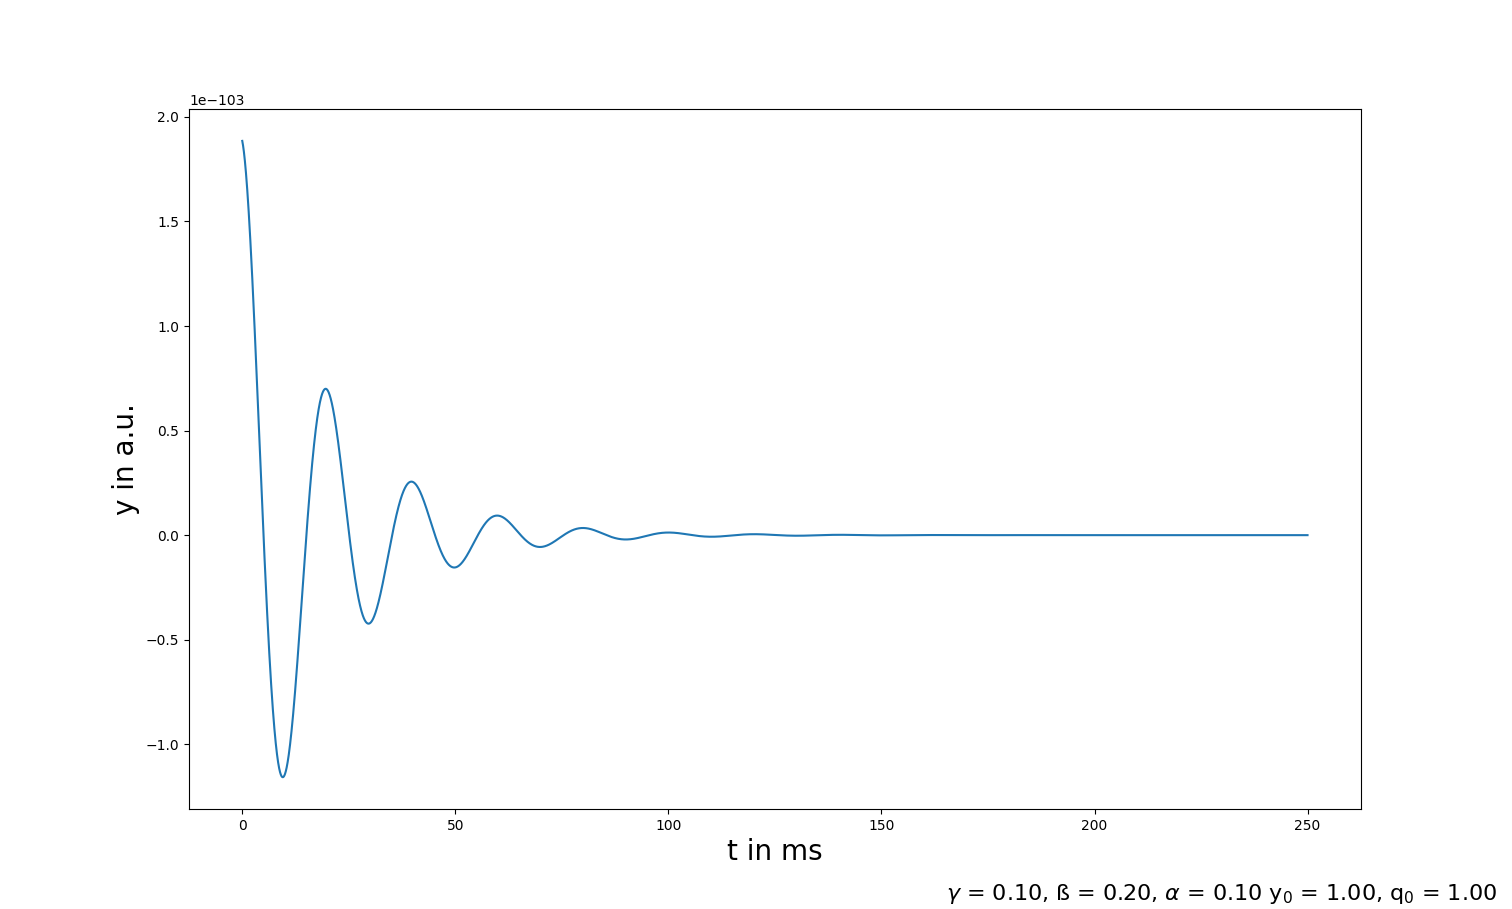
\includegraphics[scale=0.4]{duffing_unforced_y.png}
			\caption{Time series of an non-driven autonomous Duffing oscillator with the parameters $\gamma$ = 0.1, $\alpha$ = 0.1 and $\beta$ = 0.2. The resulting plot is giving by numerically integrated starting from (y,p) = (1, 1) at t = 0 ms to t = 250 ms.}
			\label{fig: duffing_unforced_y}
		\end{figure}
		
		When the Duffing oscillator is run with the given parameters, it can be observed that due to the nonlinear restoring force, the system quickly oscillates back to its equilibrium state (see Figure \ref{fig: duffing_unforced_y}).
	
	
		\section{Van der Pol Oscillator}
		The Van der Pol oscillator is also a nonlinear system, where a harmonic oscillator has been augmented with a nonlinear damping term $\mu(x^2 - 1)\dot{x}$ (see Equation \ref{eq: unforced_vdp}).\\
		The starting point for the time series was taken from the book Nonlinear Dynamics and Chaos\cite{Nonlinear_Dynamic_and_chaos_book}.
		
		\begin{equation}\label{eq: unforced_vdp}
			\frac{d^2x}{dt^2} - \mu (1 - x^2) \frac{dx}{dt} + x = 0
		\end{equation}
		\\
		The Van der Pol oscillator can self-excite and transition into a stable limit cycle. In Table \ref{tab: vdp_ungetriebene_parameter}, $\mu$ = 0.1 was chosen to keep the nonlinear damping low, allowing the system to behave similarly to a harmonic oscillator, as seen in Figure \ref{fig: vdp_unforced_x}.
		
			\begin{table}[H]
			\centering
			\caption{The meaning of the Van der Pol parameters and choosen values for them without units.}
			\label{tab: vdp_ungetriebene_parameter}
			\begin{tabular}{c c c}
				\toprule
				parameter & meaning & value\\
				\midrule
				$\mu$ & damping term & 0.1\\
				\bottomrule
			\end{tabular}
		\end{table}
		
			\begin{figure}[H]
			\centering
			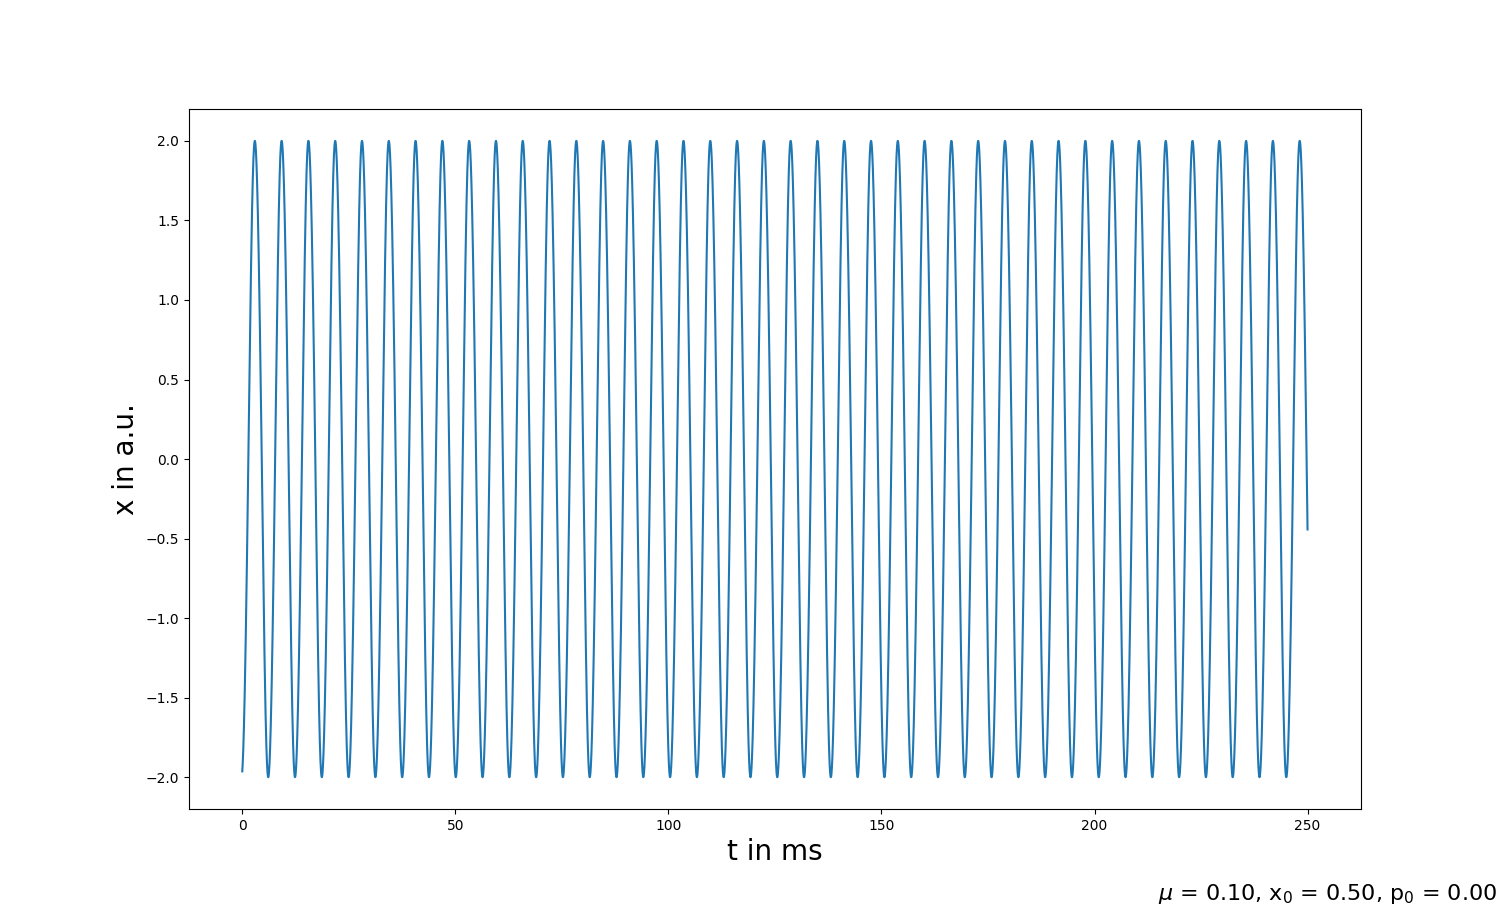
\includegraphics[scale=0.4]{vdp_unforced_x.png}
			\caption{Time series of an non-driven autonomous Van der Pol oscillator with the parameter $\mu$ = 0.1 The resulting plot is giving by numerically integrated starting from (x,q) = (0.5, 0)\cite{Nonlinear_Dynamic_and_chaos_book}. at t = 0 ms to t = 250 ms. 0.}
			\label{fig: vdp_unforced_x}
		\end{figure}
		
		
		\chapter{Implementing a new Oscillator-model}
		In Chapter \ref{chapter: Duffing- and Van der Pol Oscillator}, the uncoupled, non-driven oscillators were introduced. But what happens if the properties of both autonomous oscillators are coupled in a new differential equation? For the initial implementation, the Duffing oscillator (y(t)) is additively coupled with the Van der Pol oscillator (x(t)) using the coupling term k (see Equation \ref{eq: vdp_duffing_ODE}). As a result, the two oscillators drive each other and form a non-autonomous system.
		\begin{equation}\label{eq: vdp_duffing_ODE}
			\begin{split}
				\frac{d^2x}{dt^2} - \mu (1 - x^2) \frac{dx}{dt} + x = k ( y- x )\\
				\frac{d^2y}{dt^2} + \gamma \frac{dy}{dt} + \alpha y + \beta y^3 = k ( x-y )\\
			\end{split}
		\end{equation}
		\\
		The solution of the coupled ODE is shown in Equation \ref{eq: vdp_duffing_Lösung}.
			\begin{equation}\label{eq: vdp_duffing_Lösung}		
			\begin{gathered}
				\frac{dx}{dt} = p\\
				\frac{dp}{dt} = \mu (1 - x^2) p - x +k ( y- x )\\
				\\
				\frac{dy}{dt} = q\\
				\frac{dq}{dt} = - \gamma q - \alpha y - \beta y^3 + k ( x-y )\\
			\end{gathered}		
		\end{equation}
		\\
		For the parameters, the values from Table \ref{tab: duffing_ungetriebene_parameter} and \ref{tab: vdp_ungetriebene_parameter} were retained. A time series was numerically integrated for k = 0.0, 0.01, 0.1, 0.5, 1.0.\\
		 Due to the coupling of the two autonomous oscillators, the amplitude of the Van der Pol oscillator decreases with increasing k, while the amplitude of the Duffing oscillator increases. \\
		 The simulation was intentionally conducted only for k < 1 to minimize chaotic behavior. In Table \ref{tab: freq_x} and \ref{tab: freq_y}, the period T, frequency f, angular frequency $\omega$, and amplitude A were determined from the simulation in Figure \ref{fig: timekurve_k}. It can be seen that for the Van der Pol oscillator, the values decrease, while for the Duffing system, they increase with increasing k values.
		
		\begin{figure}[H]
			\centering
			\begin{subfigure}[b]{0.45\textwidth}
				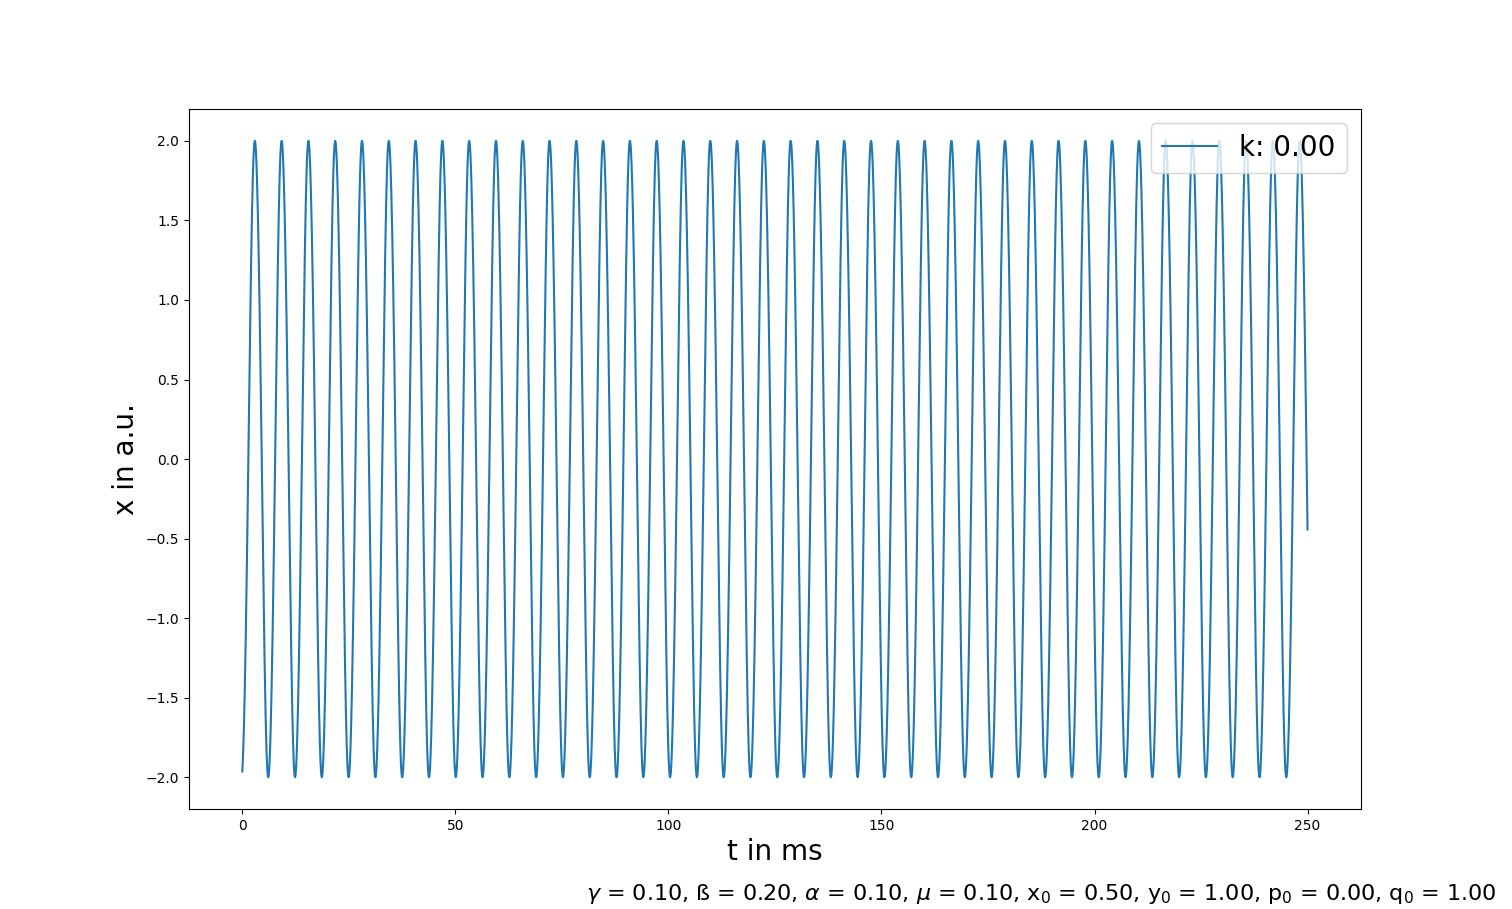
\includegraphics[width=\textwidth]{x_k1.png}
				\caption{}
				\label{fig:x1}
			\end{subfigure}
			\hfill
			\begin{subfigure}[b]{0.45\textwidth}
				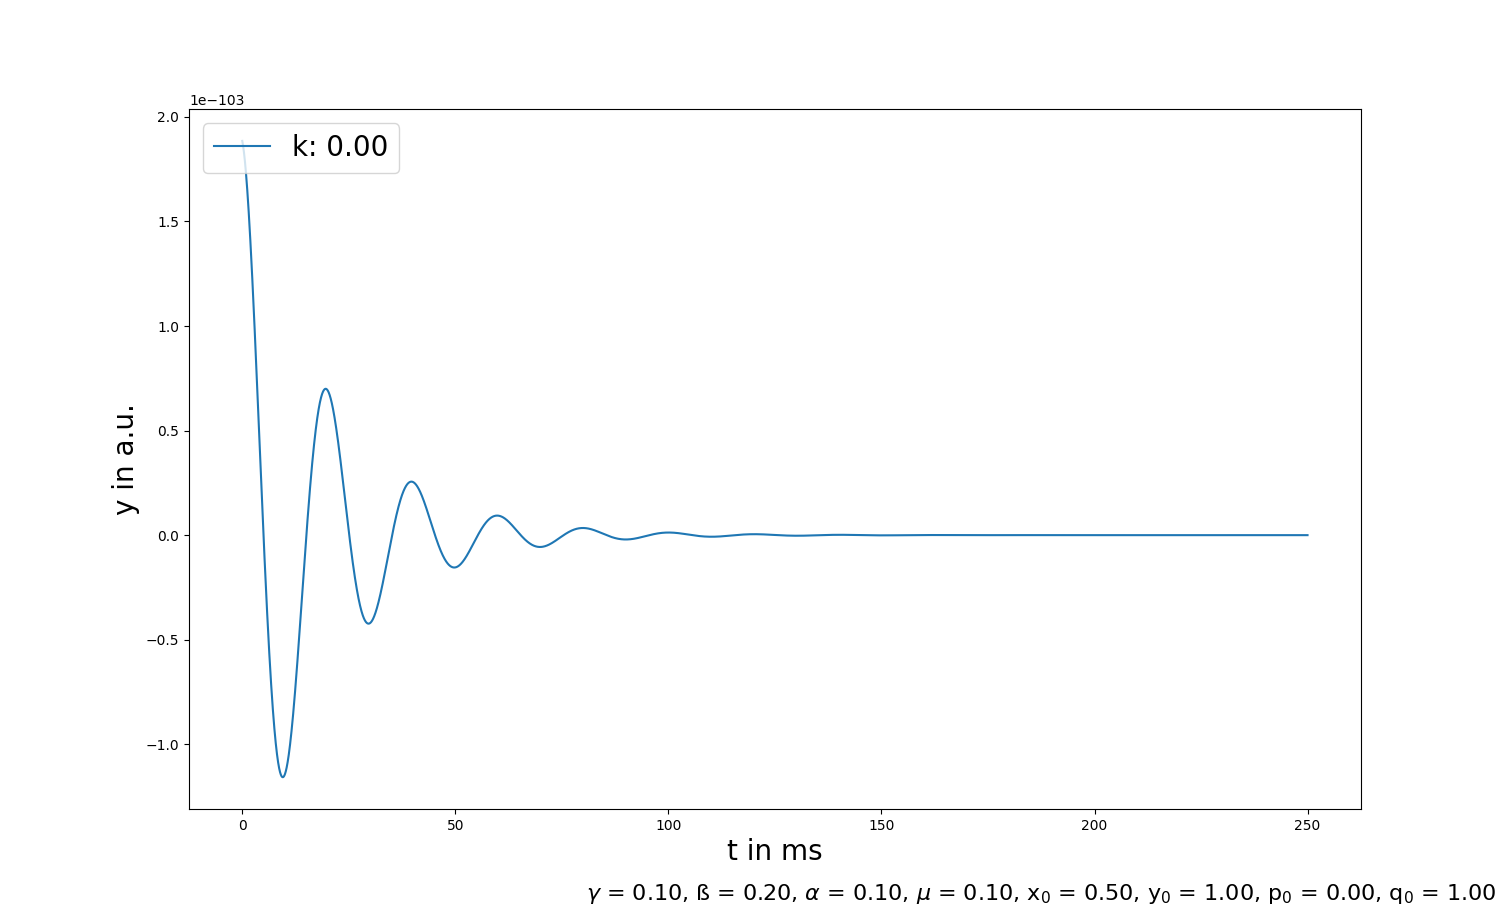
\includegraphics[width=\textwidth]{y_k1.png}
				\caption{}
				\label{fig: y1}
			\end{subfigure}
				\begin{subfigure}[b]{0.45\textwidth}
				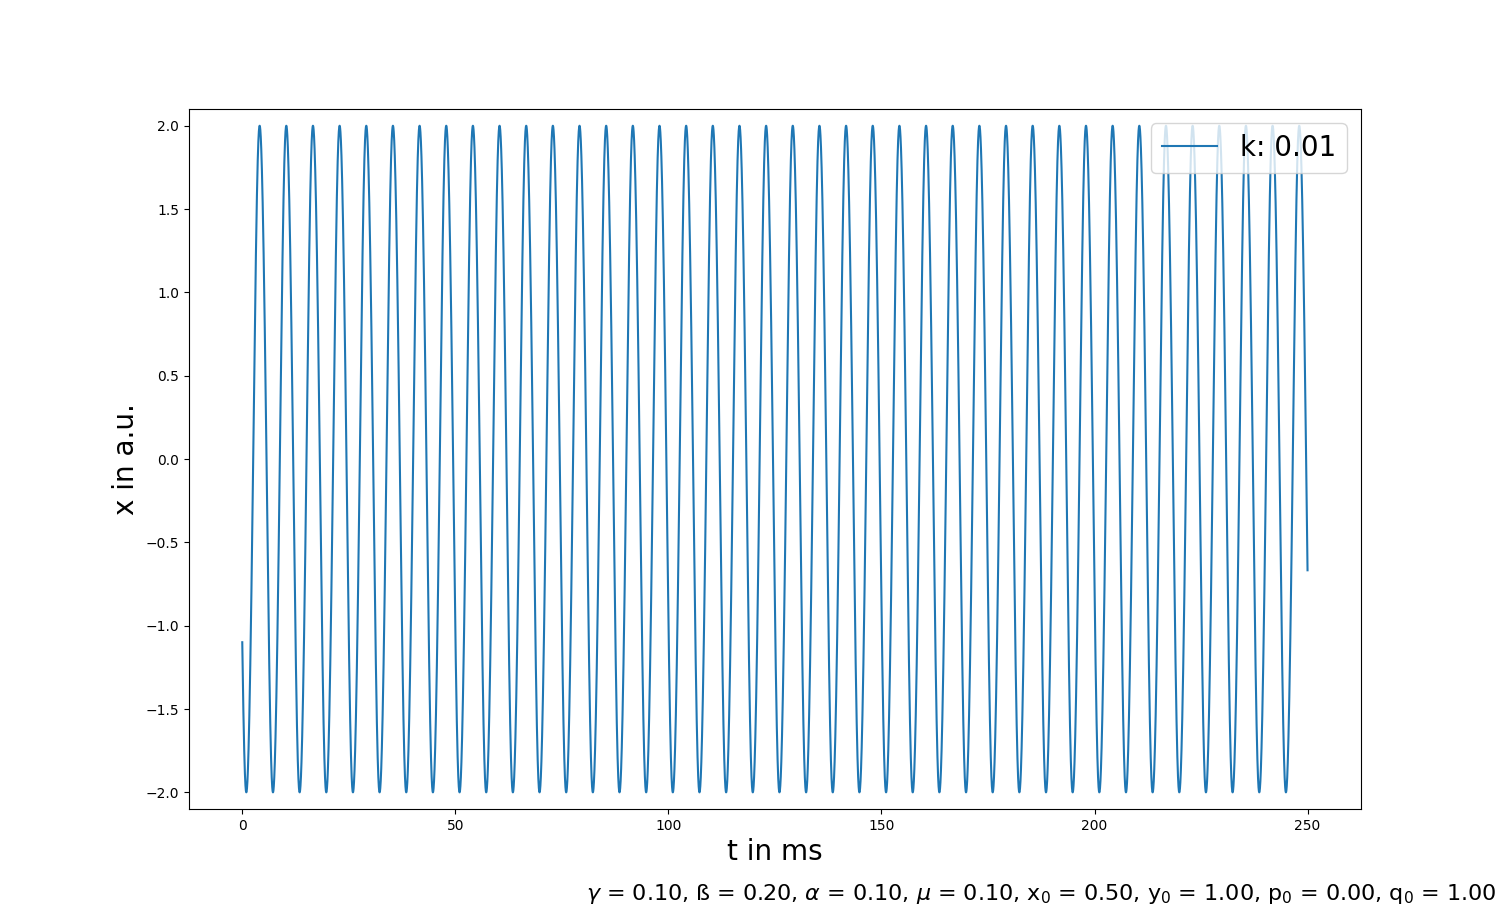
\includegraphics[width=\textwidth]{x_k5.png}
				\caption{}
				\label{fig:x5}
			\end{subfigure}
			\hfill
			\begin{subfigure}[b]{0.45\textwidth}
				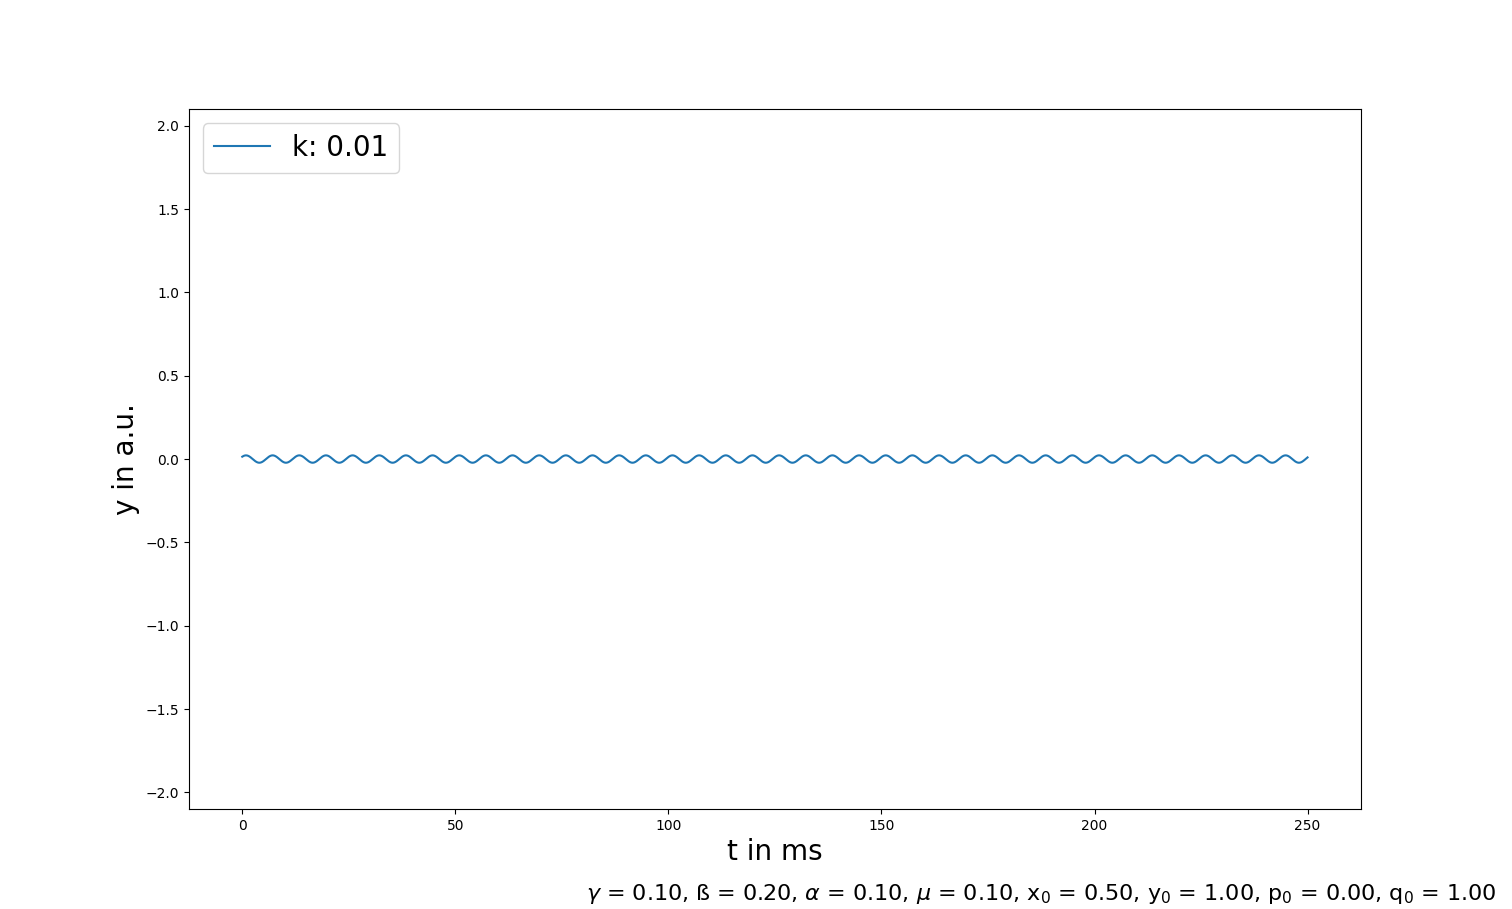
\includegraphics[width=\textwidth]{y_k5.png}
				\caption{}
				\label{fig: y5}
			\end{subfigure}
			\begin{subfigure}[b]{0.45\textwidth}
				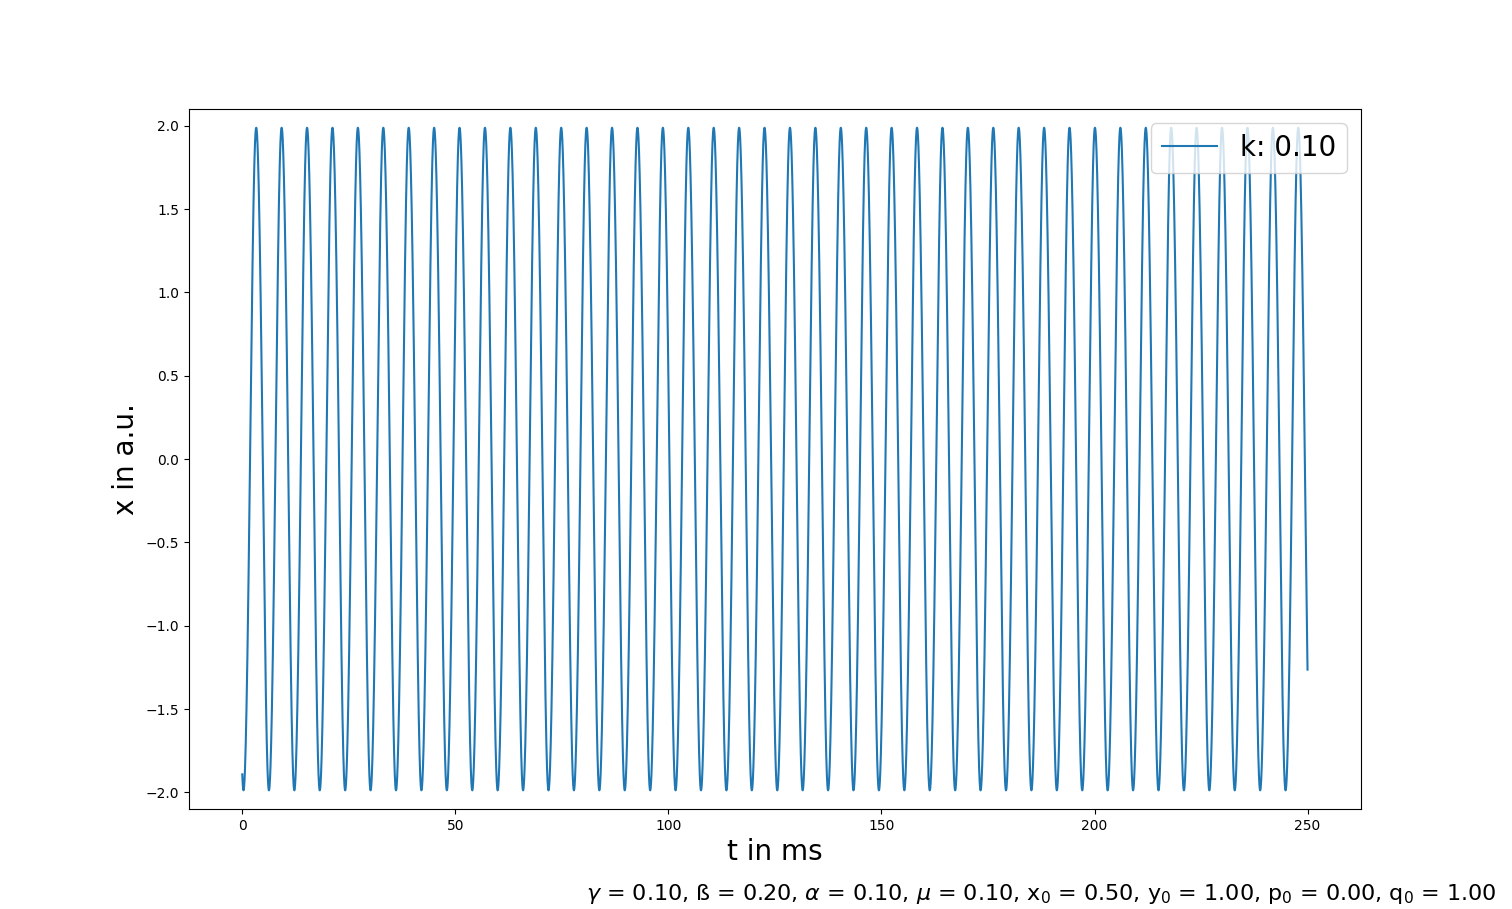
\includegraphics[width=\textwidth]{x_k2.png}
				\caption{}
				\label{fig:x2}
			\end{subfigure}
			\hfill
			\begin{subfigure}[b]{0.45\textwidth}
				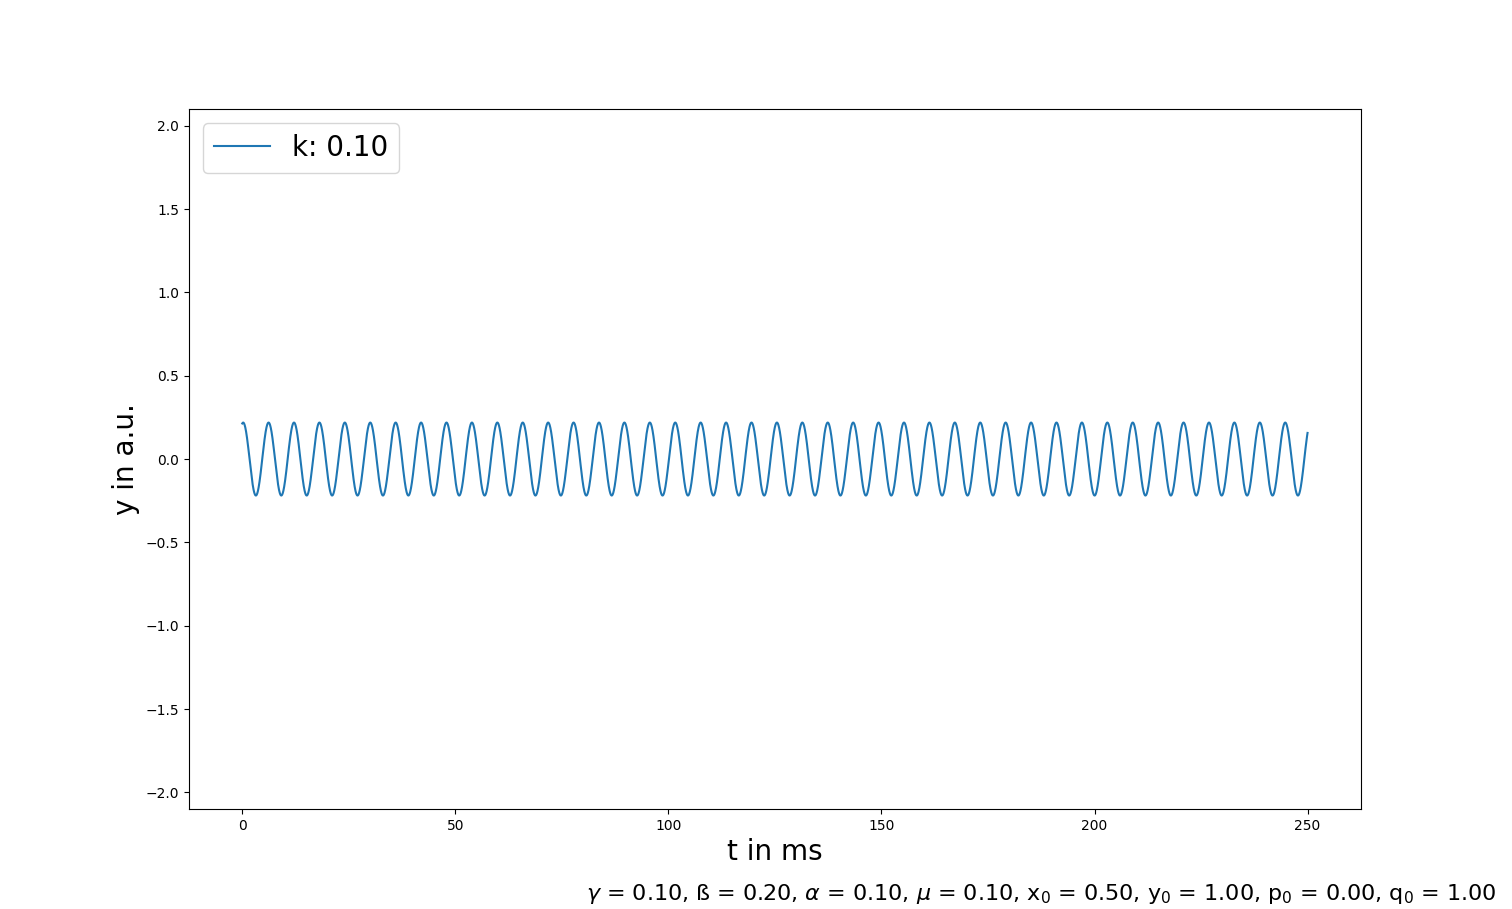
\includegraphics[width=\textwidth]{y_k2.png}
				\caption{}
				\label{fig: y2}
			\end{subfigure}
			\begin{subfigure}[b]{0.45\textwidth}
				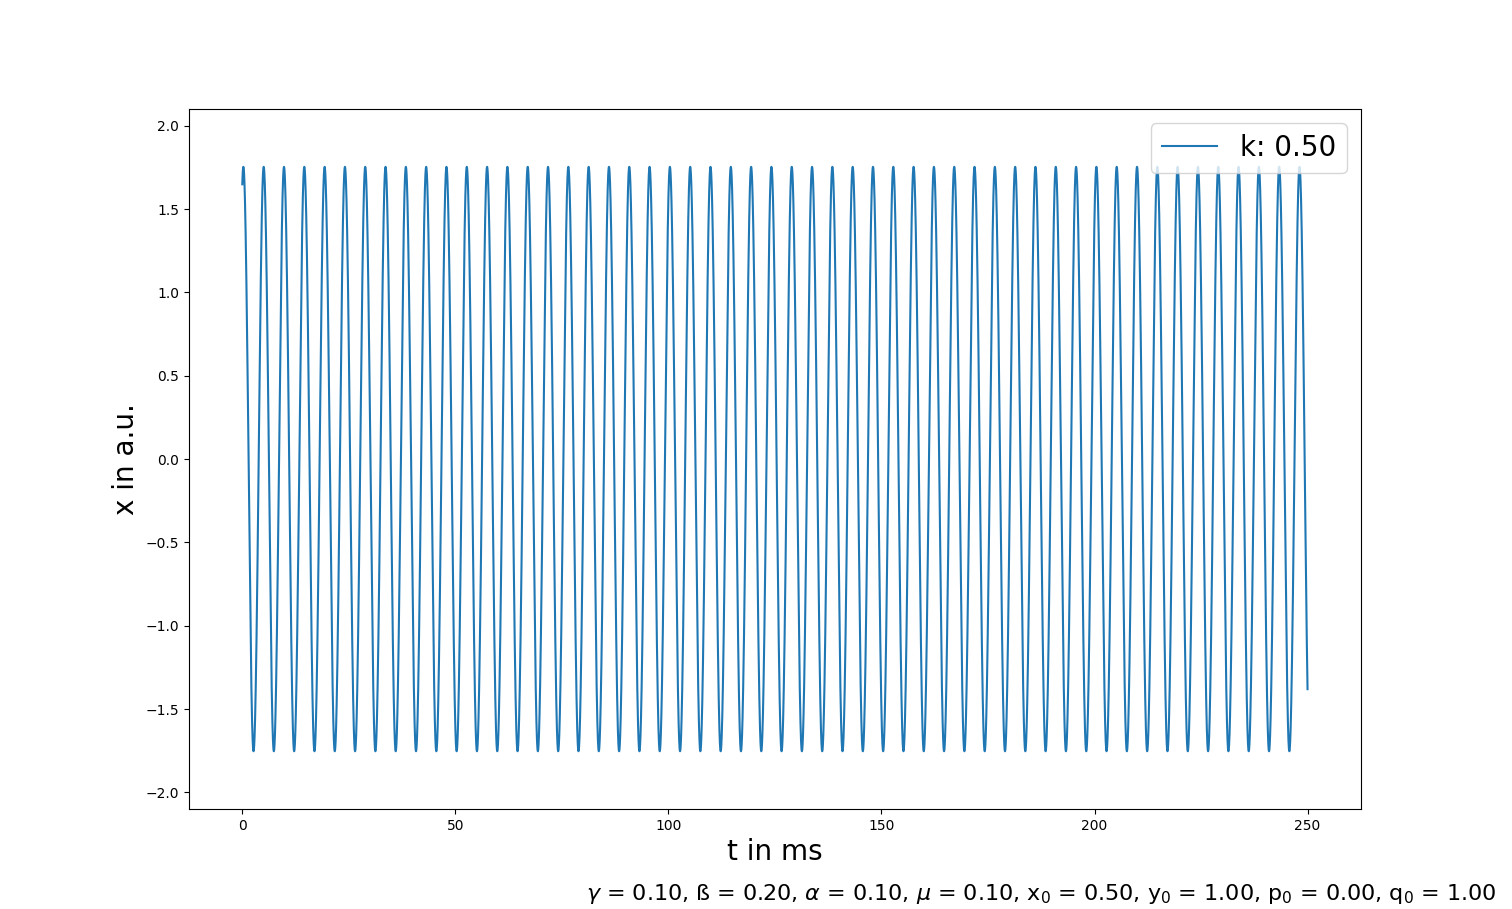
\includegraphics[width=\textwidth]{x_k3.png}
				\caption{}
				\label{fig:x3}
			\end{subfigure}
			\hfill
			\begin{subfigure}[b]{0.45\textwidth}
				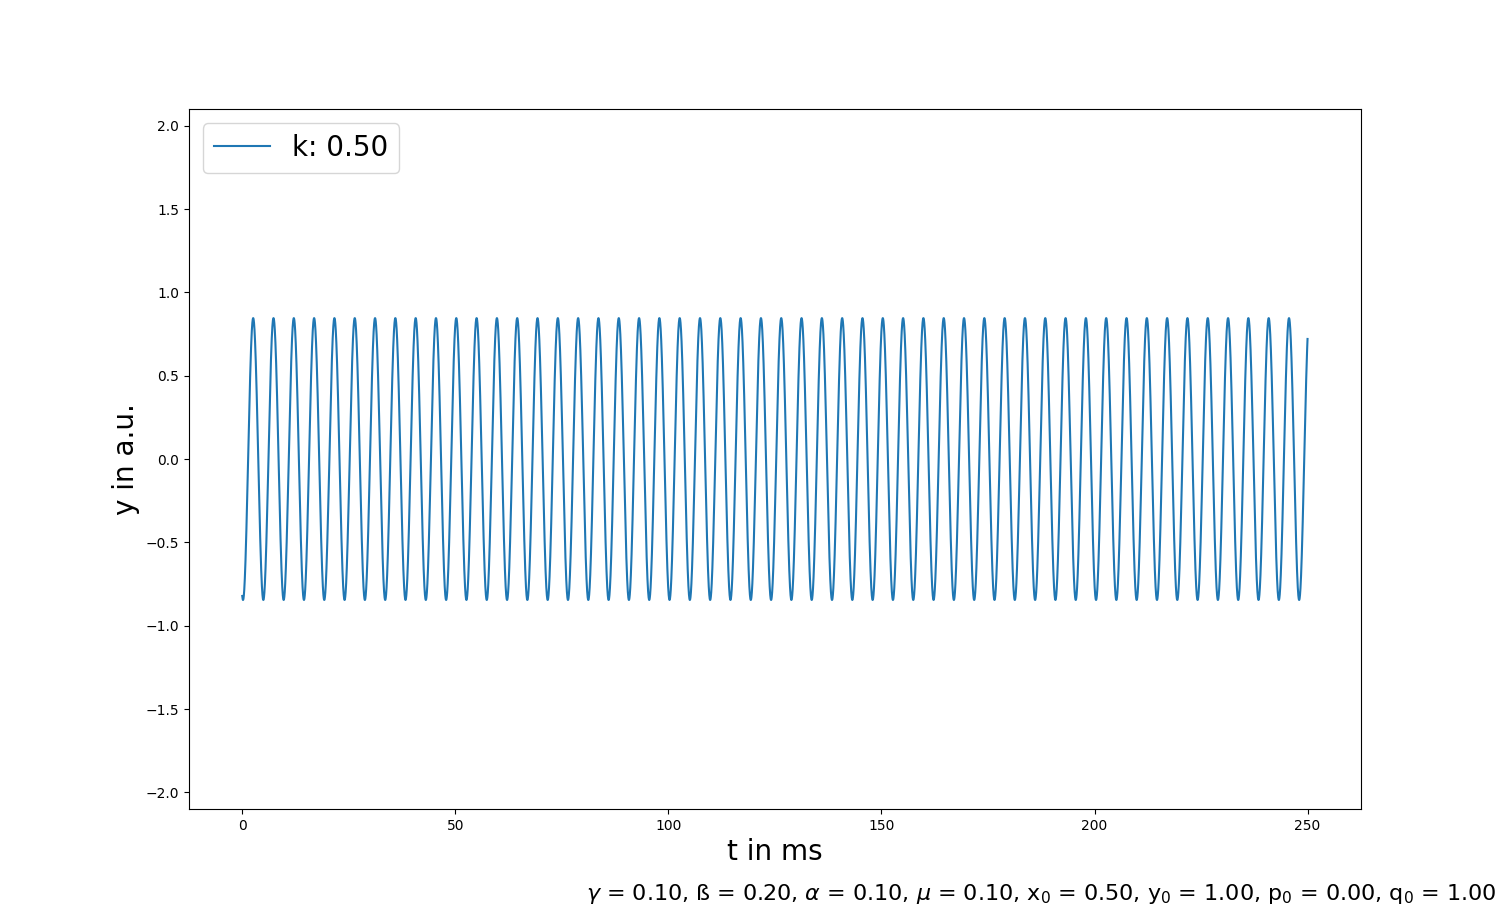
\includegraphics[width=\textwidth]{y_k3.png}
				\caption{}
				\label{fig: y3}
			\end{subfigure}
			\begin{subfigure}[b]{0.45\textwidth}
				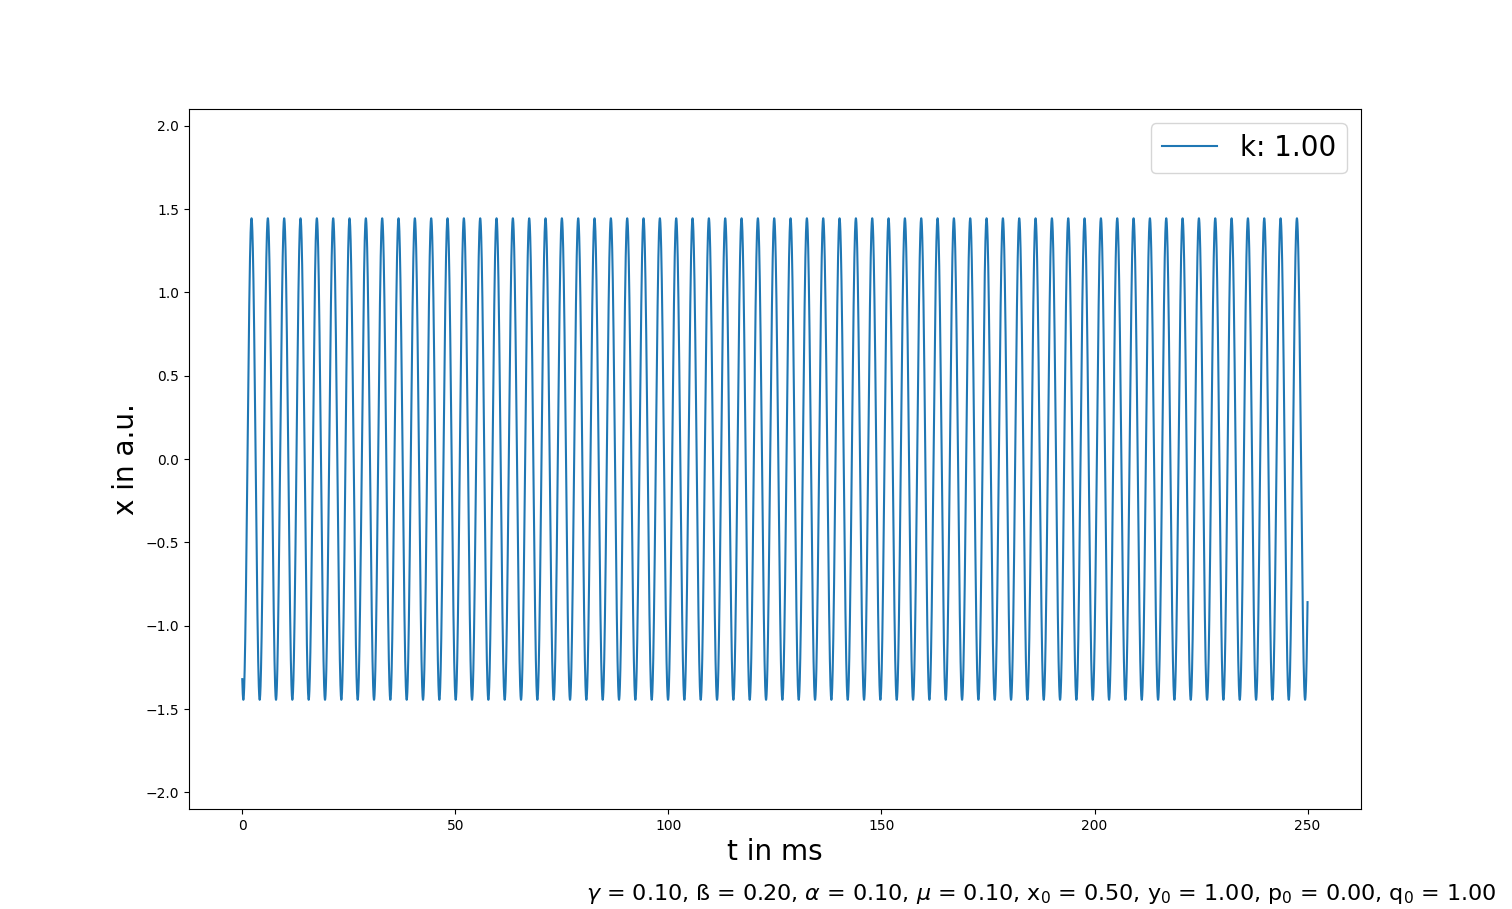
\includegraphics[width=\textwidth]{x_k4.png}
				\caption{}
				\label{fig:x4}
			\end{subfigure}
			\hfill
			\begin{subfigure}[b]{0.45\textwidth}
				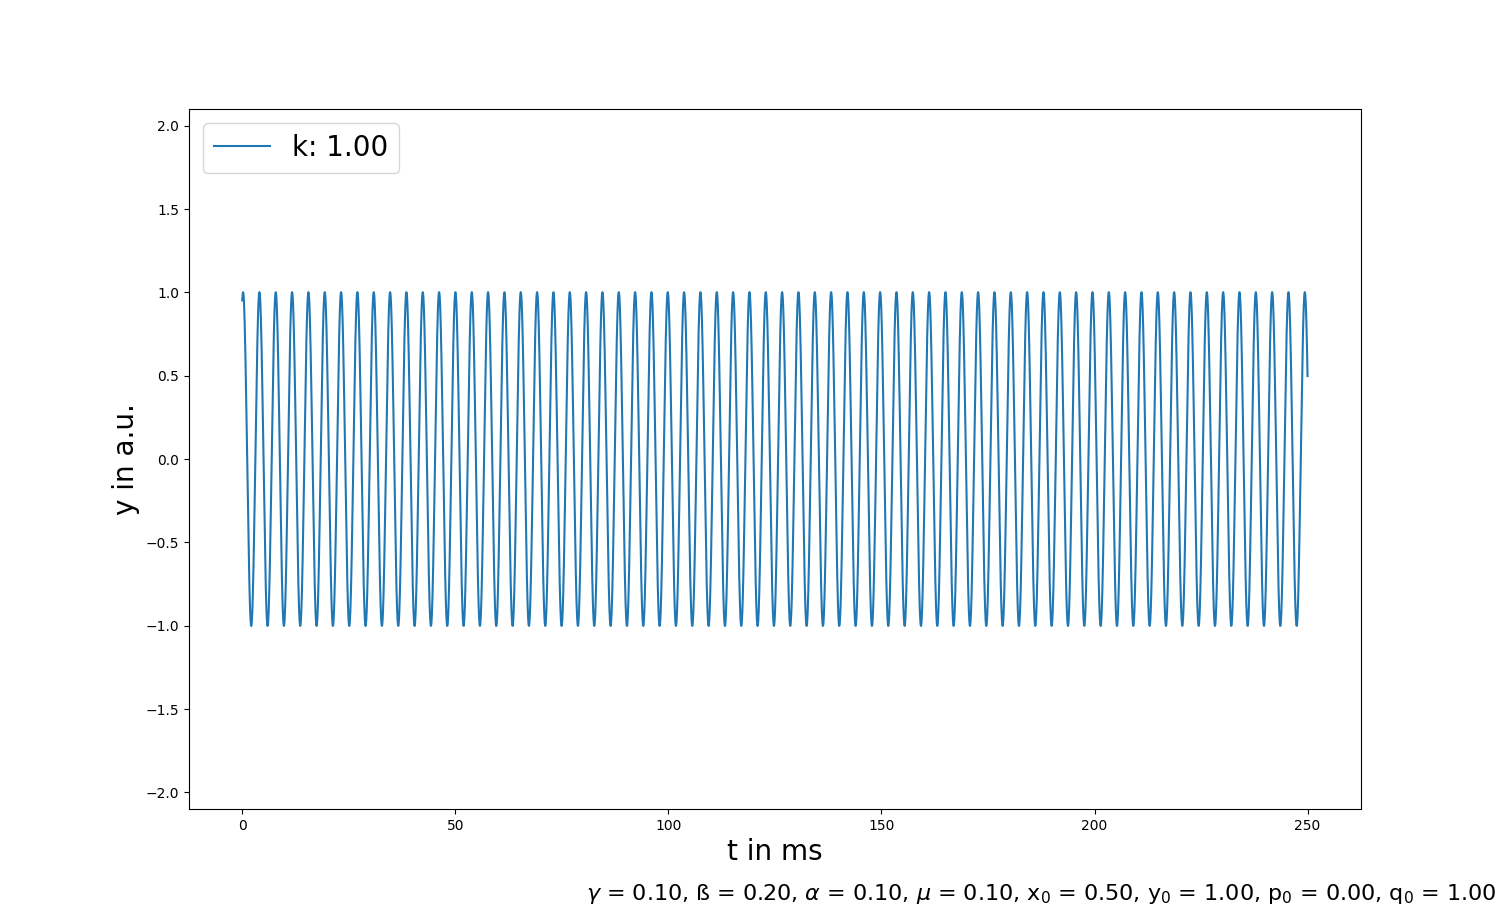
\includegraphics[width=\textwidth]{y_k4.png}
				\caption{}
				\label{fig: y4}
			\end{subfigure}
			\caption{Simulation of the additively coupled Duffing/Van der Pol oscillators as a time series for for t = [0, 250] ms. 
				The simulation was conducted with the following parameters: $\gamma$ = 0.1, $\alpha$ = 0.1 and $\beta$ = 0.2, $\mu$ = 0.1. The giving Startingpoint for this simulation is (x, q, y,p) = (0.5, 0.0, 1.0, 1.0).
				 (\ref{fig:x1}, \ref{fig: y1}) for k = 0.0, (\ref{fig:x5}, \ref{fig: y5}) for k = 0.01,(\ref{fig:x2}, \ref{fig: y2}) for k = 0.1, (\ref{fig:x3}, \ref{fig: y3}) for k = 0.5, (\ref{fig:x4}, \ref{fig: y4} ) for k = 1.0}
			\label{fig: timekurve_k}
		\end{figure}
		
		\begin{table}[H]
			\centering
			\caption{Additively coupled Van der Pol Oscillator x: Period T, Frequency f, angular frequency $\omega$ and Amplitude A for k = 0.00, 0.01, 0.10, 0.50, 1.00.}
			\label{tab: freq_x}
			\begin{tabular}{c c c c c}
				\toprule
				k & Period T & Frequency f & $\omega$ & Amplitude A \\
				\midrule
				0.00 & 6.29 & 0.16 & 1.00 & 2.00 \\
				0.01 & 6.26 & 0.16 & 1.00 & 1.99 \\
				0.10 & 5.96 & 0.17 & 1.05 & 1.98 \\
				0.50 & 4.79 & 0.21 & 1.31 & 1.71 \\
				1.00 & 3.90 & 0.26 & 1.61 & 1.37 \\
				\bottomrule
			\end{tabular}
		\end{table}
		\begin{table}[H]
			\centering
			\caption{Additively coupled Duffing Oscillator y: Period T, Frequency f, angular frequency $\omega$ and Amplitude A for k = 0.00, 0.01, 0.10, 0.50, 1.00.}
			\label{tab: freq_y}
			\begin{tabular}{c c c c c}
				\toprule
				k & Period T & Frequency f & $\omega$ & Amplitude A \\
				\midrule
				0.00 &19.92 & 0.05 & 0.32 & - \\
				0.01 & 6.38 & 0.16 & 0.98 & 0.03 \\
				0.10 & 6.01 & 0.17 & 1.05 & 0.23 \\
				0.50 & 4.80 & 0.21 & 1.31 & 0.84 \\
				1.00 & 3.92 & 0.26 & 1.60 & 0.96 \\
				\bottomrule
			\end{tabular}
		\end{table}
		
		With a very small coupling constant of 
		k = 0.01, the Duffing oscillator can be driven to a self-sustained oscillator. The resonance curve of the Duffing oscillator can be observed in Figure \ref{fig:resonanz}. At 
		k = 0.01 , a resonance curve is obtained that shows a strong resonance frequency \ref{fig:resonanz2}, exhibiting behavior similar to that of a linear system. When the system is not coupled with another force, no resonance is observed \ref{fig:resonanz1}. As 
		k approaches the value of 1, more complex resonance behavior emerges, which requires further investigation (see Figure \ref{fig:resonanz3}, \ref{fig: resonanz4}, \ref{fig:resonanz5}).
	\begin{figure}[H]
		\centering
		\begin{subfigure}[b]{0.45\textwidth}
			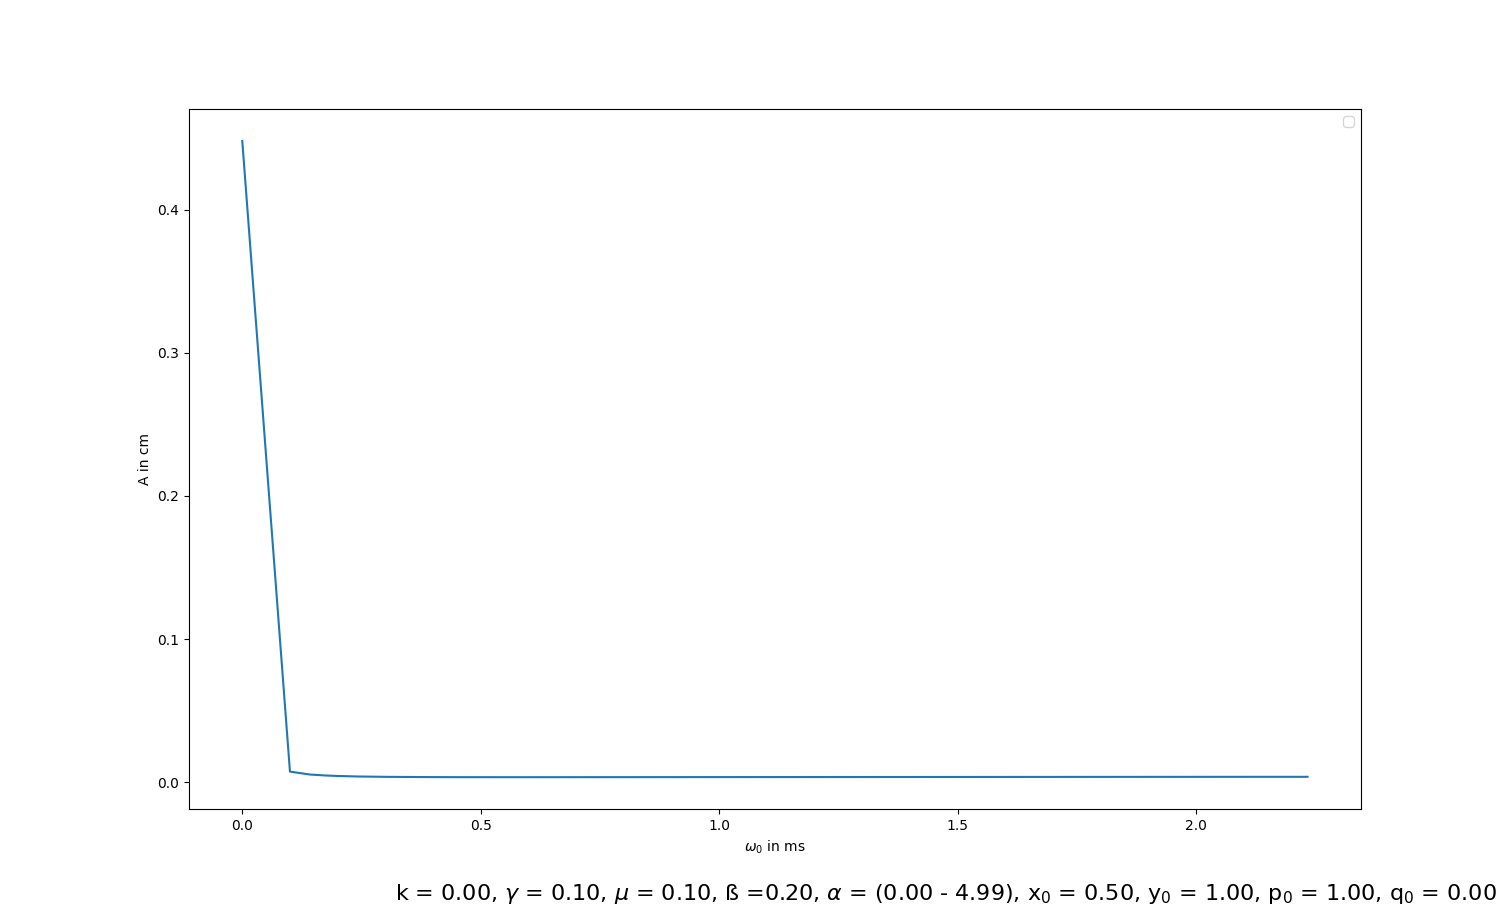
\includegraphics[width=\textwidth]{resonanz1.png}
			\caption{}
			\label{fig:resonanz1}
		\end{subfigure}
		\hfill
		\begin{subfigure}[b]{0.45\textwidth}
			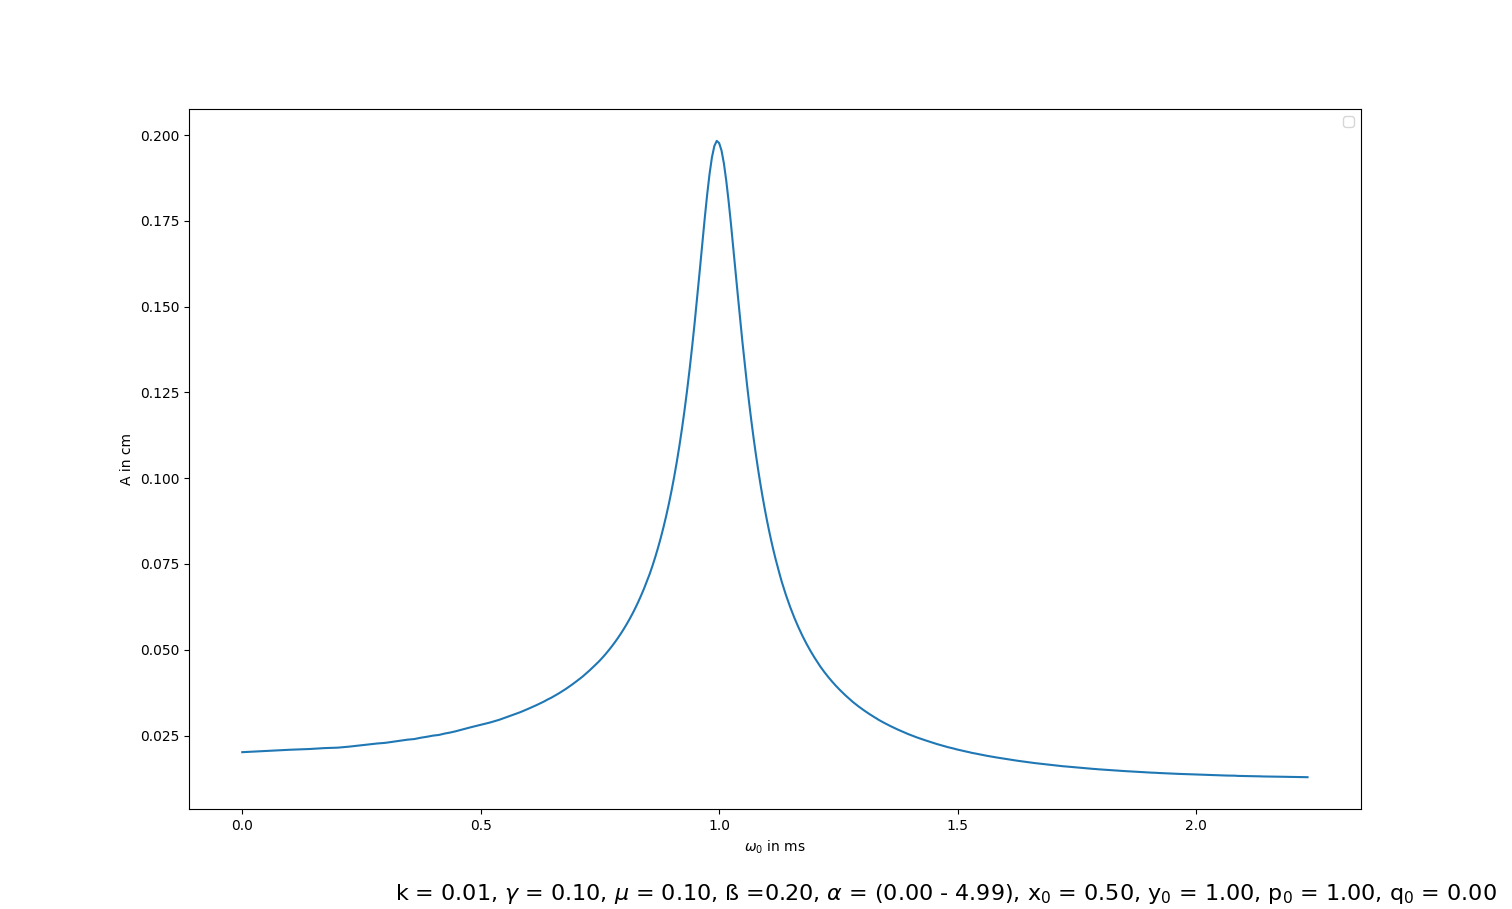
\includegraphics[width=\textwidth]{resonanz2.png}
			\caption{}
			\label{fig:resonanz2}
		\end{subfigure}
		\begin{subfigure}[b]{0.45\textwidth}
			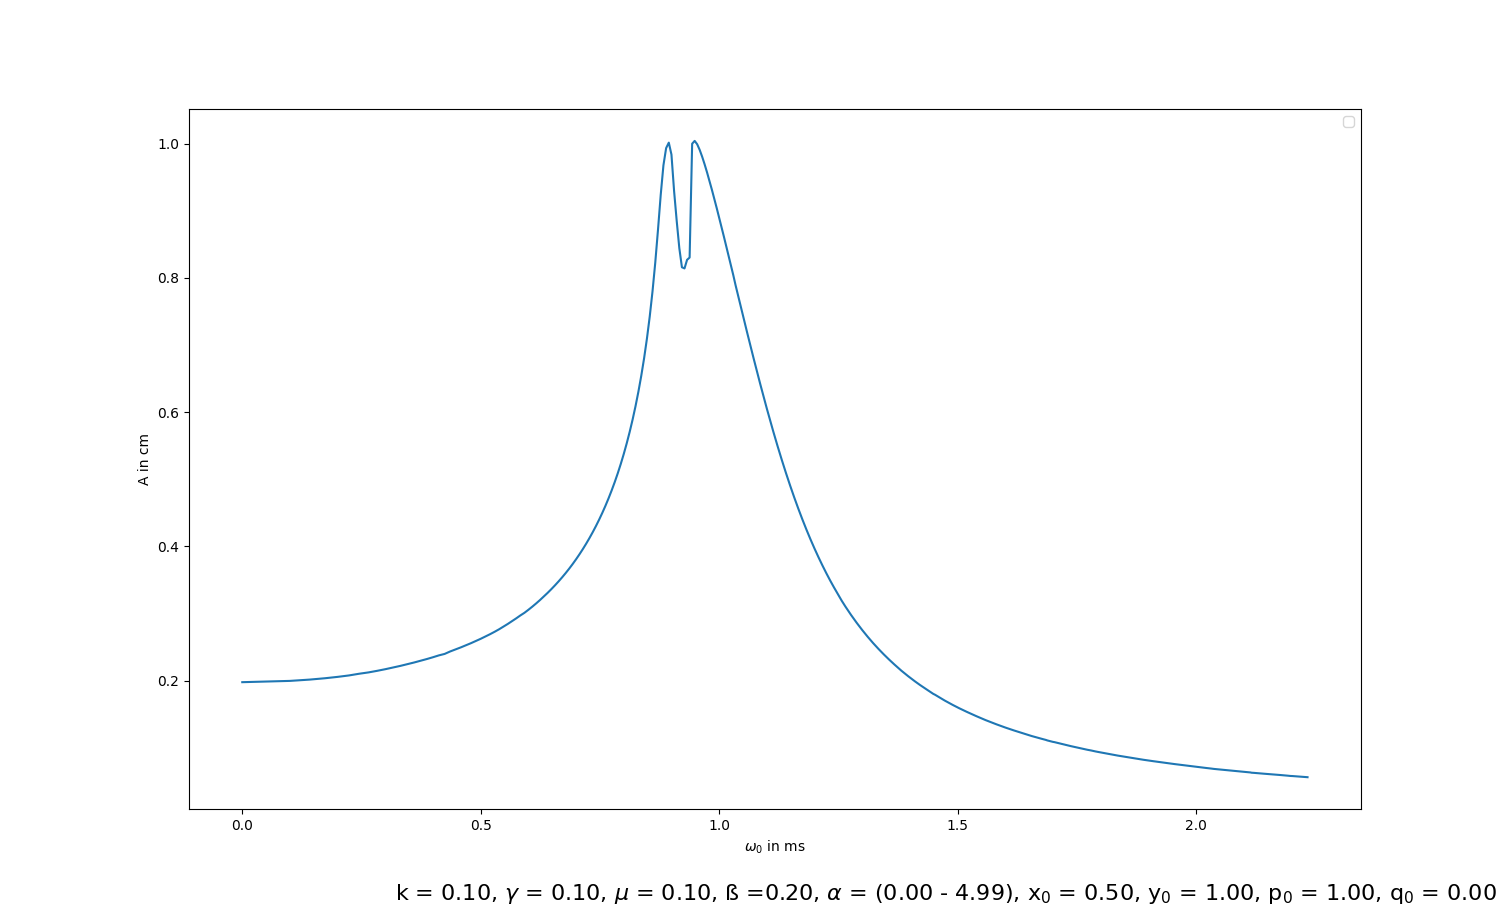
\includegraphics[width=\textwidth]{resonanz3.png}
			\caption{}
			\label{fig:resonanz3}
		\end{subfigure}
		\hfill
		\begin{subfigure}[b]{0.45\textwidth}
			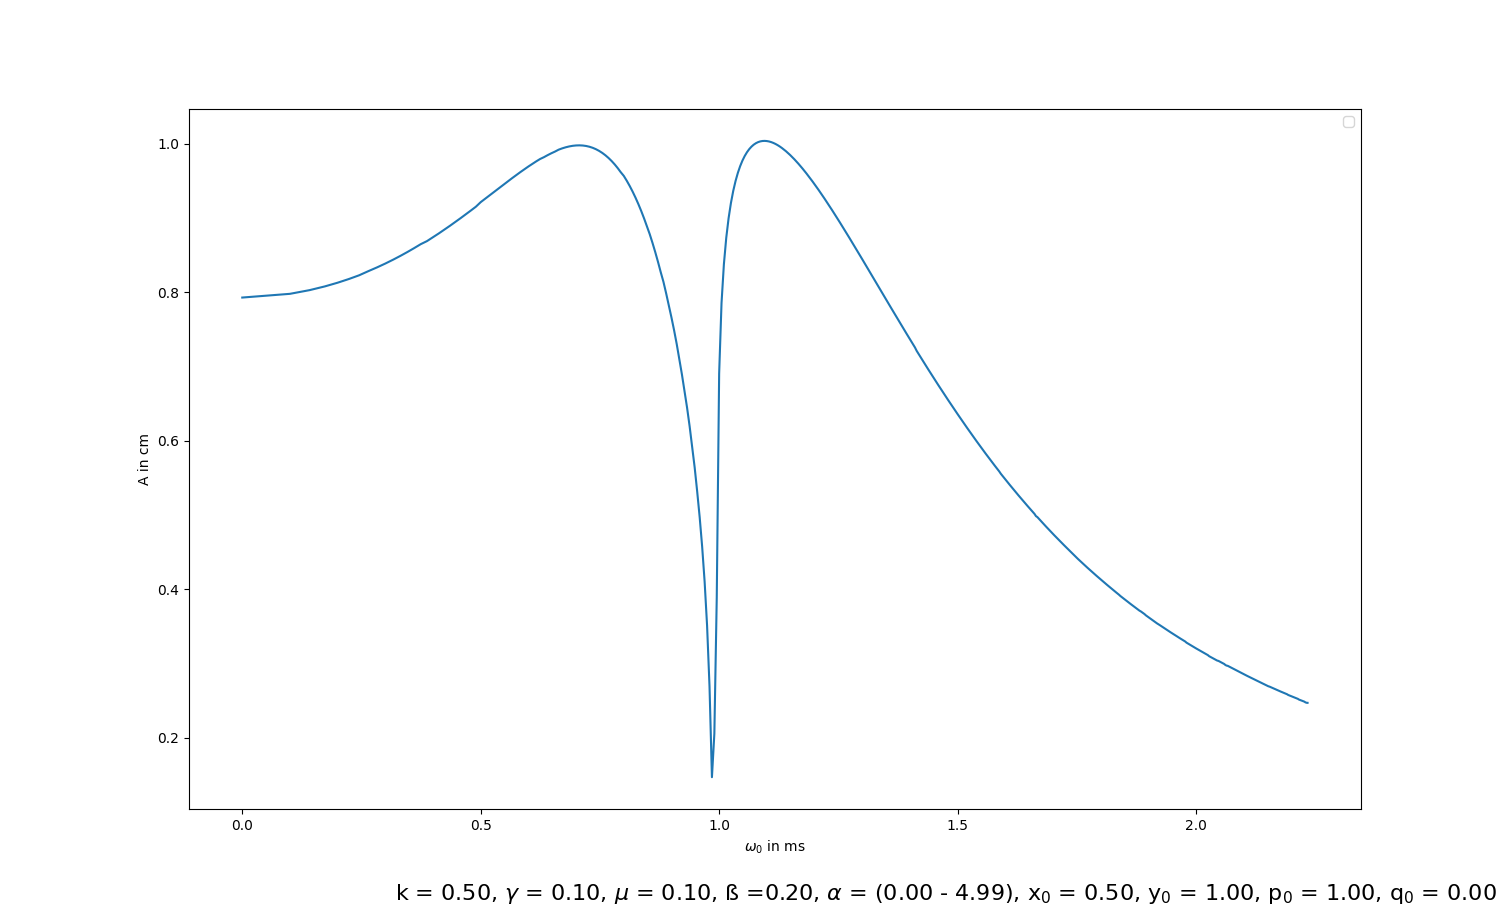
\includegraphics[width=\textwidth]{resonanz4.png}
			\caption{}
			\label{fig: resonanz4}
		\end{subfigure}
		\begin{subfigure}[b]{0.45\textwidth}
			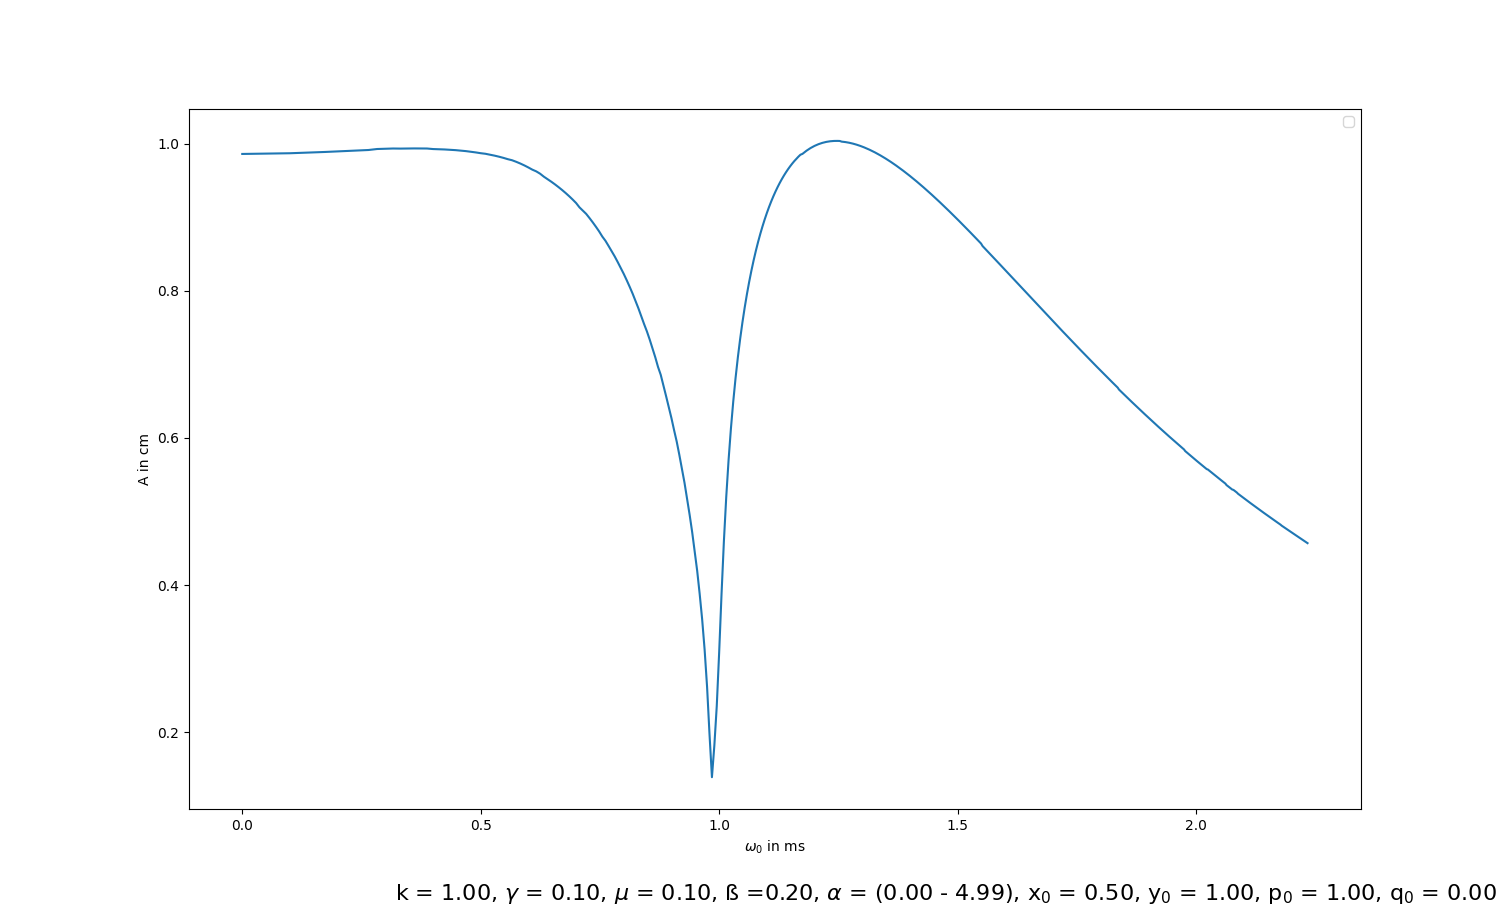
\includegraphics[width=\textwidth]{resonanz5.png}
			\caption{}
			\label{fig:resonanz5}
		\end{subfigure}
		
		\caption{Amplitude response of Duffing oscillator driven by Van der Pol oscillator. The coupling constant k are 0.00, 0.01, 0.10, 0.50 and 1.00 for the giving parameters: $\gamma$ = 0.1, $\alpha$ = (0.00 - 5.00) and $\beta$ = 0.2, $\mu$ = 0.1. The giving Startingpoint for this simulation is (x, q, y,p) = (0.5, 0.0, 1.0, 1.0).}
		\label{fig:resonanz}
	\end{figure}
		
		
	\chapter{Outlook}	
		As seen in this small chapter, much remains to be understood about the new oscillator model. What happens when the coupling constant k exceeds 1? What values should the individual parameters take to represent certain behaviors? What chaotic behavior can be observed here? Are bifurcations detectable, and can a truly nonlinear sound production like that described by Daniel Priegnitz be explained through simple additive coupling of the Duffing and Van der Pol oscillators?\\
		 \\
		For my bachelor's thesis, I want to understand the chaotic behavior of the newly designed oscillator model and be able to simulate the metal vocals using the in vivo data from Daniel Priegnitz. But that might take a while. \\
		The next step for this project is to find a bifurcation in the system and then simulate the vocal folds and false vocal folds.
	\addcontentsline{toc}{chapter}{Bibliography}
	\bibliographystyle{plainurl}
	\nocite{*}
	\bibliography{Literatur}
	\newpage
\end{document}